\documentclass[11pt]{beamer}

%%% \mode must be on a line by its own, without comment or whitespace!
%%% \mode sets the mode to presentation. So if the mode is presentation the slides after are shown
%%% if the mode is not presentation (but article or handout) they are not shown
\mode<presentation>{}

\usetheme{Warsaw}
\usepackage[utf8]{inputenc}
\usepackage[english]{babel}
\usepackage{amsmath}
\usepackage{amsfonts}
\usepackage{amssymb}
\usepackage{graphicx}
\usepackage{xspace}

\author{Guus Bonnema}
\title{Final Presentation\\(XMas Designer)}
%\setbeamercovered{transparent} 
%\setbeamertemplate{navigation symbols}{} 
%\logo{} 
\institute{Open University\\team033\\Guus Bonnema, Stefan Versluys, Jeroen Kleijn} 
\date{May 20, 2015} 
\subject{XMas Designer} 

\begin{document}

\newcommand{\Noc}{\textsc{NoC}\xspace}
\newcommand{\qt}{\textsc{Qt}\xspace}
\newcommand{\qml}{\textsc{Qml}\xspace}

\begin{frame}
\titlepage
\end{frame}

\begin{frame}{Overview Iterations}
	\begin{columns}
		\begin{column}[t]{5cm}
			Process
			\begin{itemize}
				\item <1->Planning phase: DAD approach
				\item <1->Domain analyses
				\item <1->Iteration 0 Architecture
				\item <1->Iteration 1 Build procedures and first prototype
				\item <1->iteration 2, 3, 4, 5 software development
				\item <1->\textit{Final Demo}$\leftarrow$
				\item <1->\textbf{transition}
				\begin{itemize}
					\item {\tiny research context}
					\item {\tiny software release version}
					\item {\tiny final presentation}
				\end{itemize}
			\end{itemize}
		\end{column}
		\begin{column}[t]{5cm}
			Development factors
			\begin{itemize}
				\item <2,7->Time boxing
				\item <3,7->Early switch to \qt
				\item <4,5,7->UI design : \qml
				\item <5,7->Qml / xmas integration: fat interface
				\item <6,7->Reorg OU $\rightarrow$ Communication drop
			\end{itemize}
		\end{column}
	\end{columns}
\end{frame}

\begin{frame}{Specification model Data Layer iteration 1}

	\includegraphics[width=.95\linewidth]{pictures/1c-architecture-dynamic-1}

\end{frame}

\begin{frame}{Implementation Data layer}

	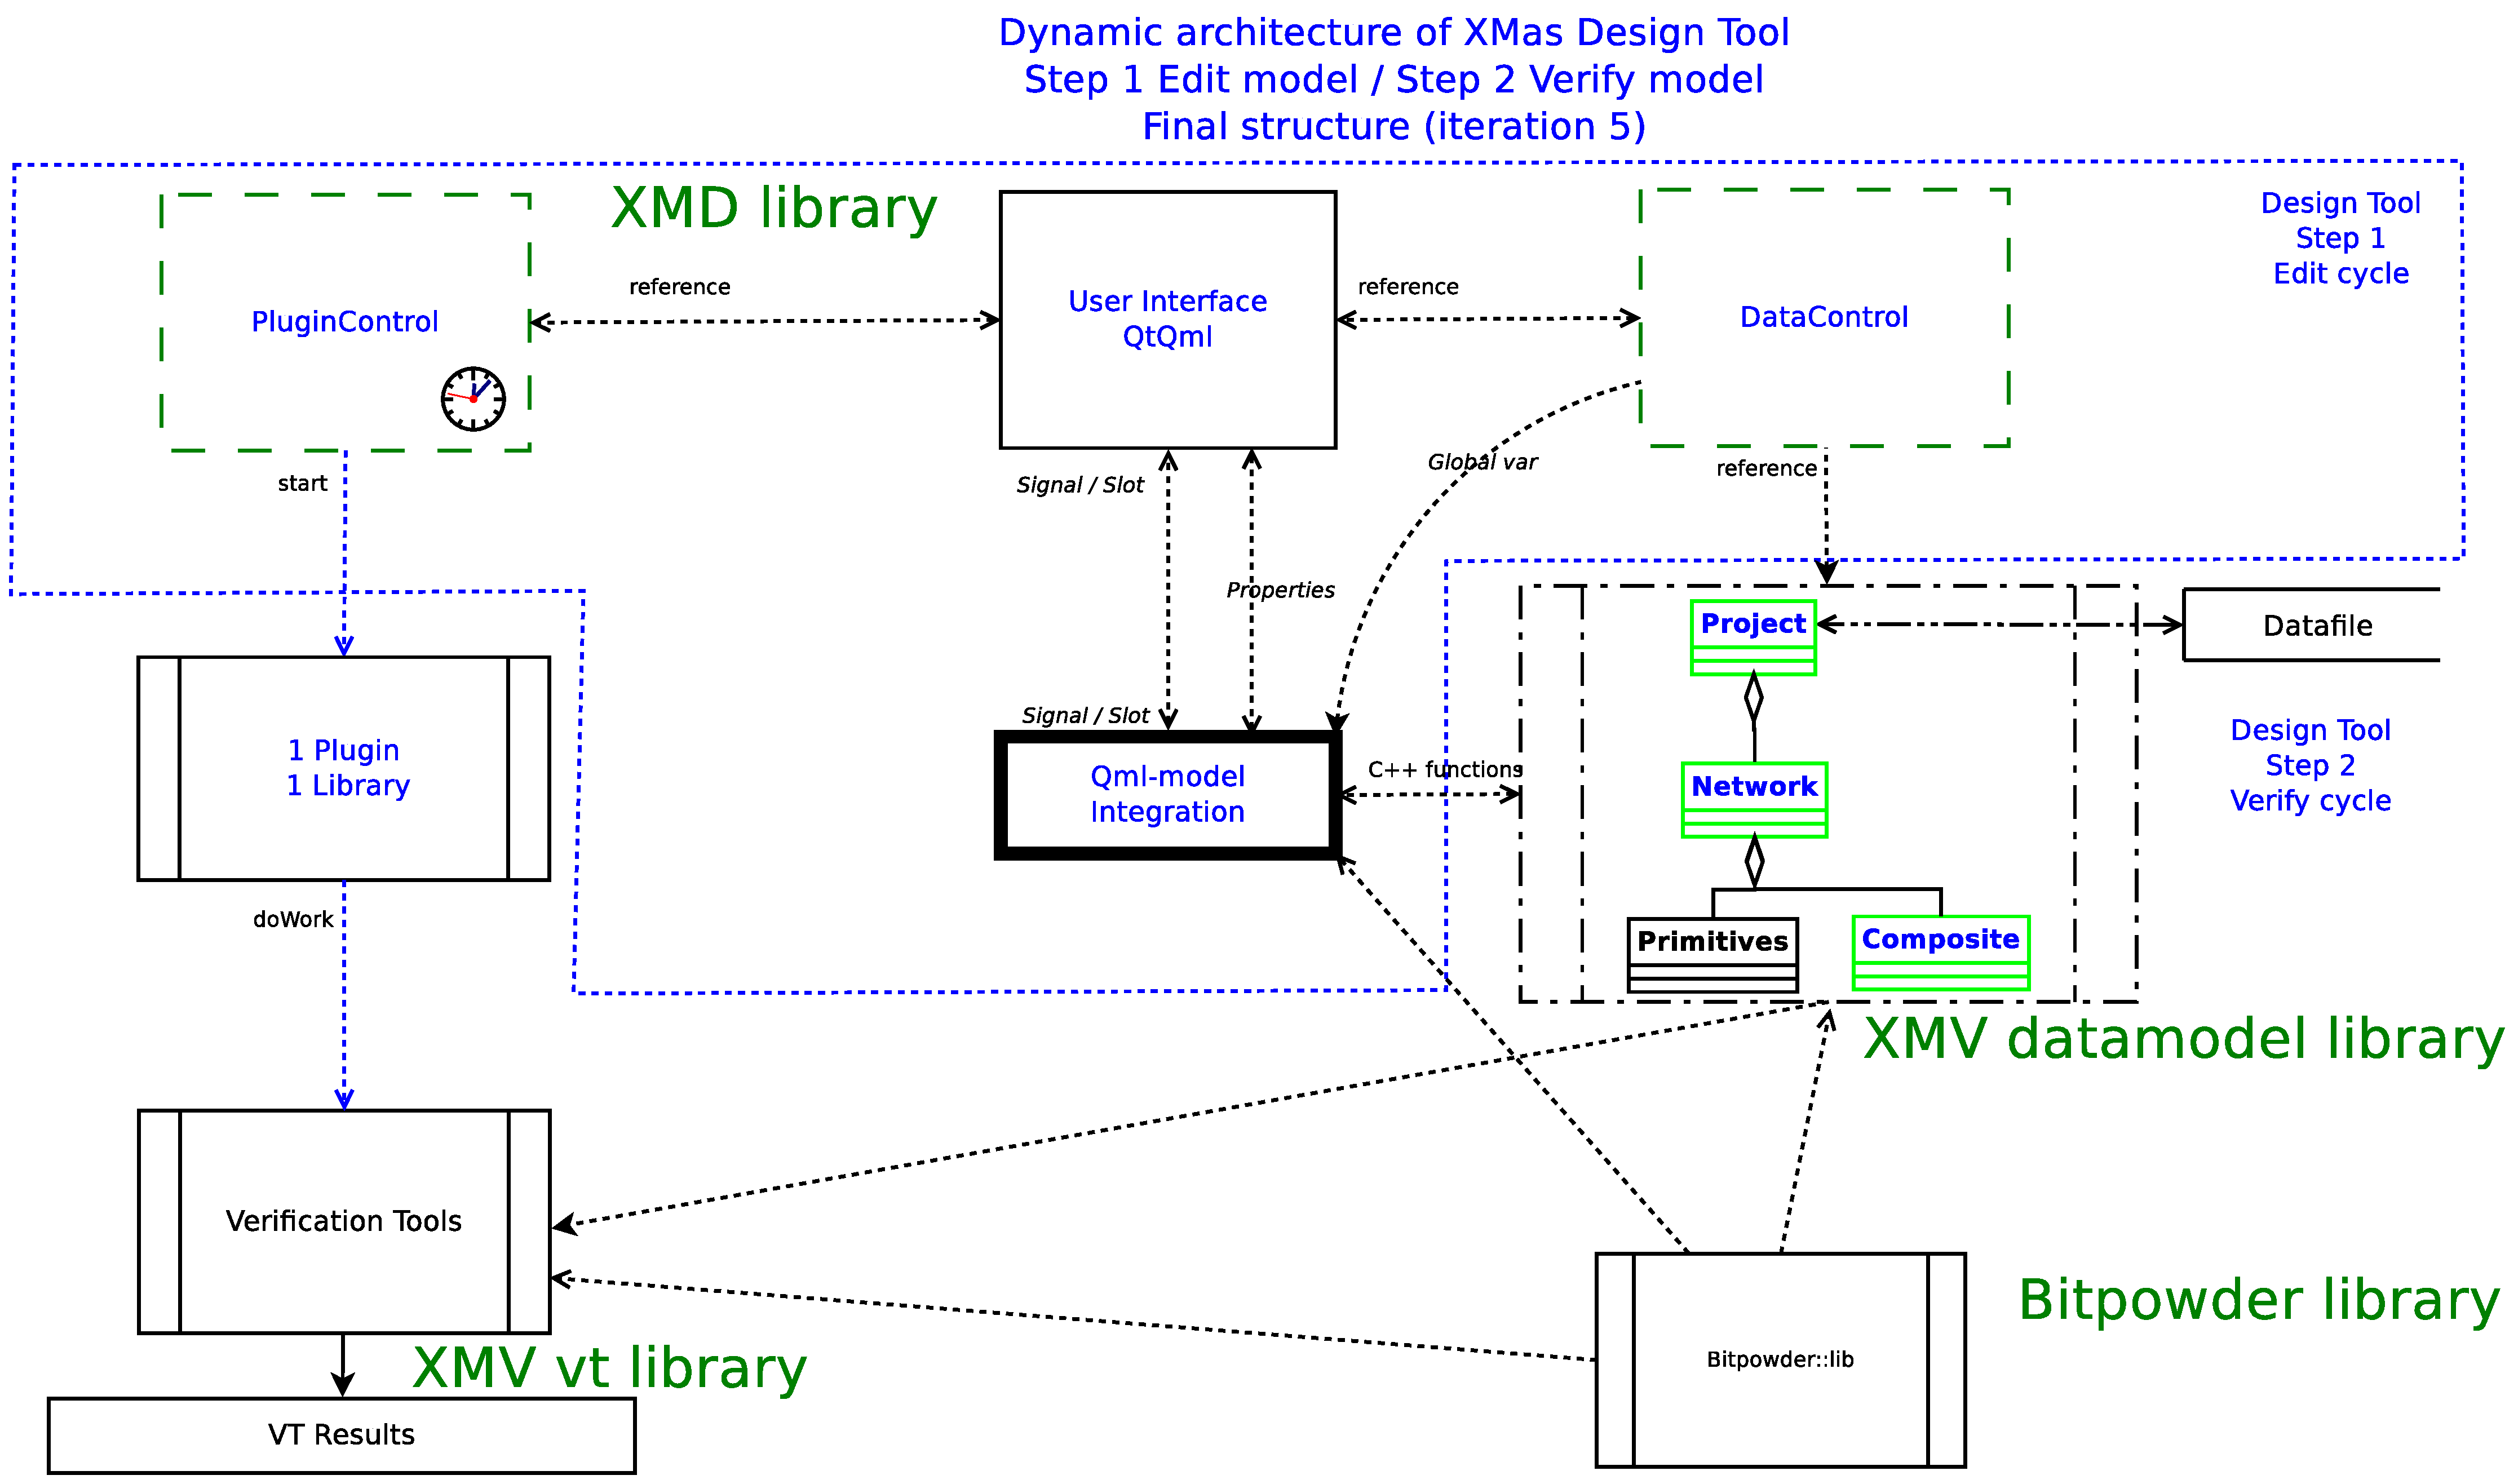
\includegraphics[width=.95\linewidth]{pictures/1c-architecture-dynamic-2}

\end{frame}

\begin{frame}{User Interface}

	\begin{itemize}
		\item Stefan : demo
	\end{itemize}

\end{frame}

\end{document}
